%%
%%
%%      SECTION: BEAM PATTERN 
%%

%% [intro]
%%________________________________________________________

The NIKA2 beam pattern mainly depends on the IRAM 30m telescope and
NIKA2 full (external and internal) optical system characteristics,
whereas the detectors themselve might have an impact at sub-dominant
level (through e.g. time constants or correlated noises).

In this section, we characterize both the main beam, which is
modeled as an elliptical Gaussian, and the full beam pattern including
error beams up to angular scales of 10 arcmin.

%% [Afternoon beam broadening ]
%%________________________________________________________
\section{Telescope-driven beam variations {\color{blue} Laurence}}
\label{se:obsdate_variations}

In this section, we evidence a beam size broadening depending on the
scan observation date. This effect, which mainly impacts late
afternoon observations and is reproducible from a campaign to another,
is probably due to deformations of the main dish subject to the Sun
heating. This is a well-known effect, which also impacts EMIR and was
observed for the previous generation of instrument MAMBO. However,
compared to the period when MAMBO or NIKA were on activity, these
daily deformations have probably strengthen due to the aging of the
main dish white coating.

\subsection{Beam monitoring using beammaps}

We monitor the time-dependent beam-size variations using all the
available beam-map scans of Uranus, Neptune and the bright quasar 3C84
acquired at the optimal focus for each campaign.
The beam size is estimated by fitting a 2D Gaussian from the map and
taking the geometrical FWHM, defined as 
$\rm{FWHM}_{\rm{geom}} = (\rm{FWHM}_x \rm{FWHM}_y)^{1/2}$, where
$\rm{FWHM}_x$ and $\rm{FWHM}_y$ are the best-fitting values of FWHM
along the minor and major axis of the elliptical 2D Gaussian. 

\addparag{Monitoring using beammaps: FIG FWHM vs obsdate, tous runs}

\subsection{Beam monitoring using pointing}

\addparag{Monitoring using pointing scans: FIG FWHM vs obsdate, tous runs}


%% [Full beam pattern]
%%________________________________________________________
\section{Full beam pattern {\color{blue} Laurence}}
\label{se:fullbeam}

\subsection{Data sets}
\label{se:beammap_set}

The characterization of the IRAM 30-m beam pattern observed through NIKA2 detectors is mainly based on observations of strong compact sources, such as planets including Uranus, Neptune and Mars, and bright quasars. We generally use beam-map scans, which we recall, are deep-integration raster-scan observations that consist of 99 sub-scans placed at intervals of $4.8''$ to cover a total of $13.5' \times 7.8'$. Most of our beam-related analysis are beased on the same set of beam-map scans as previously selected to perform the average FOV reconstruction. The set comprises nine beam-map scans that distribute as one from N2R8, '20170125s243', two from N2R9, '20170224s177' and '20170226s415' and six from N2R10, which are '20170226s425', '20170227s84', '20170419s133', '20170420s113', '20170424s116', '20170424s123'. 


\subsection{Deep beam maps}
\label{se:beammaps}
We present the two-dimensional distribution of the beam in Fig.~\ref{fig:beam}. We primary use a map obtained from a combination of deep observations of strong point sources collected during \emph{NIKA2-run8} and \emph{run9}. Namely, we use 'beammap' OTF scans of Uranus (scan id '20170125s223' and '20170125s243'),  Neptune ('20170224s177') and the bright quasar 3C84 ('20170226s415'). However, we checked the stability of our results on single scan maps, combinations of scans for a single source, and combinations of shallower scans but spanning a large range of scanning direction. The data processing includes a mitigation of the correlated noise, which mainly originates from the atmosphere.  We primarly use a subtraction of a common mode estimated from the most correlated detectors (the so-called 'cm one block' method). However, other methods are tested for assessing the immunity of our results to noise residuals.

\begin{figure}
\begin{center}
  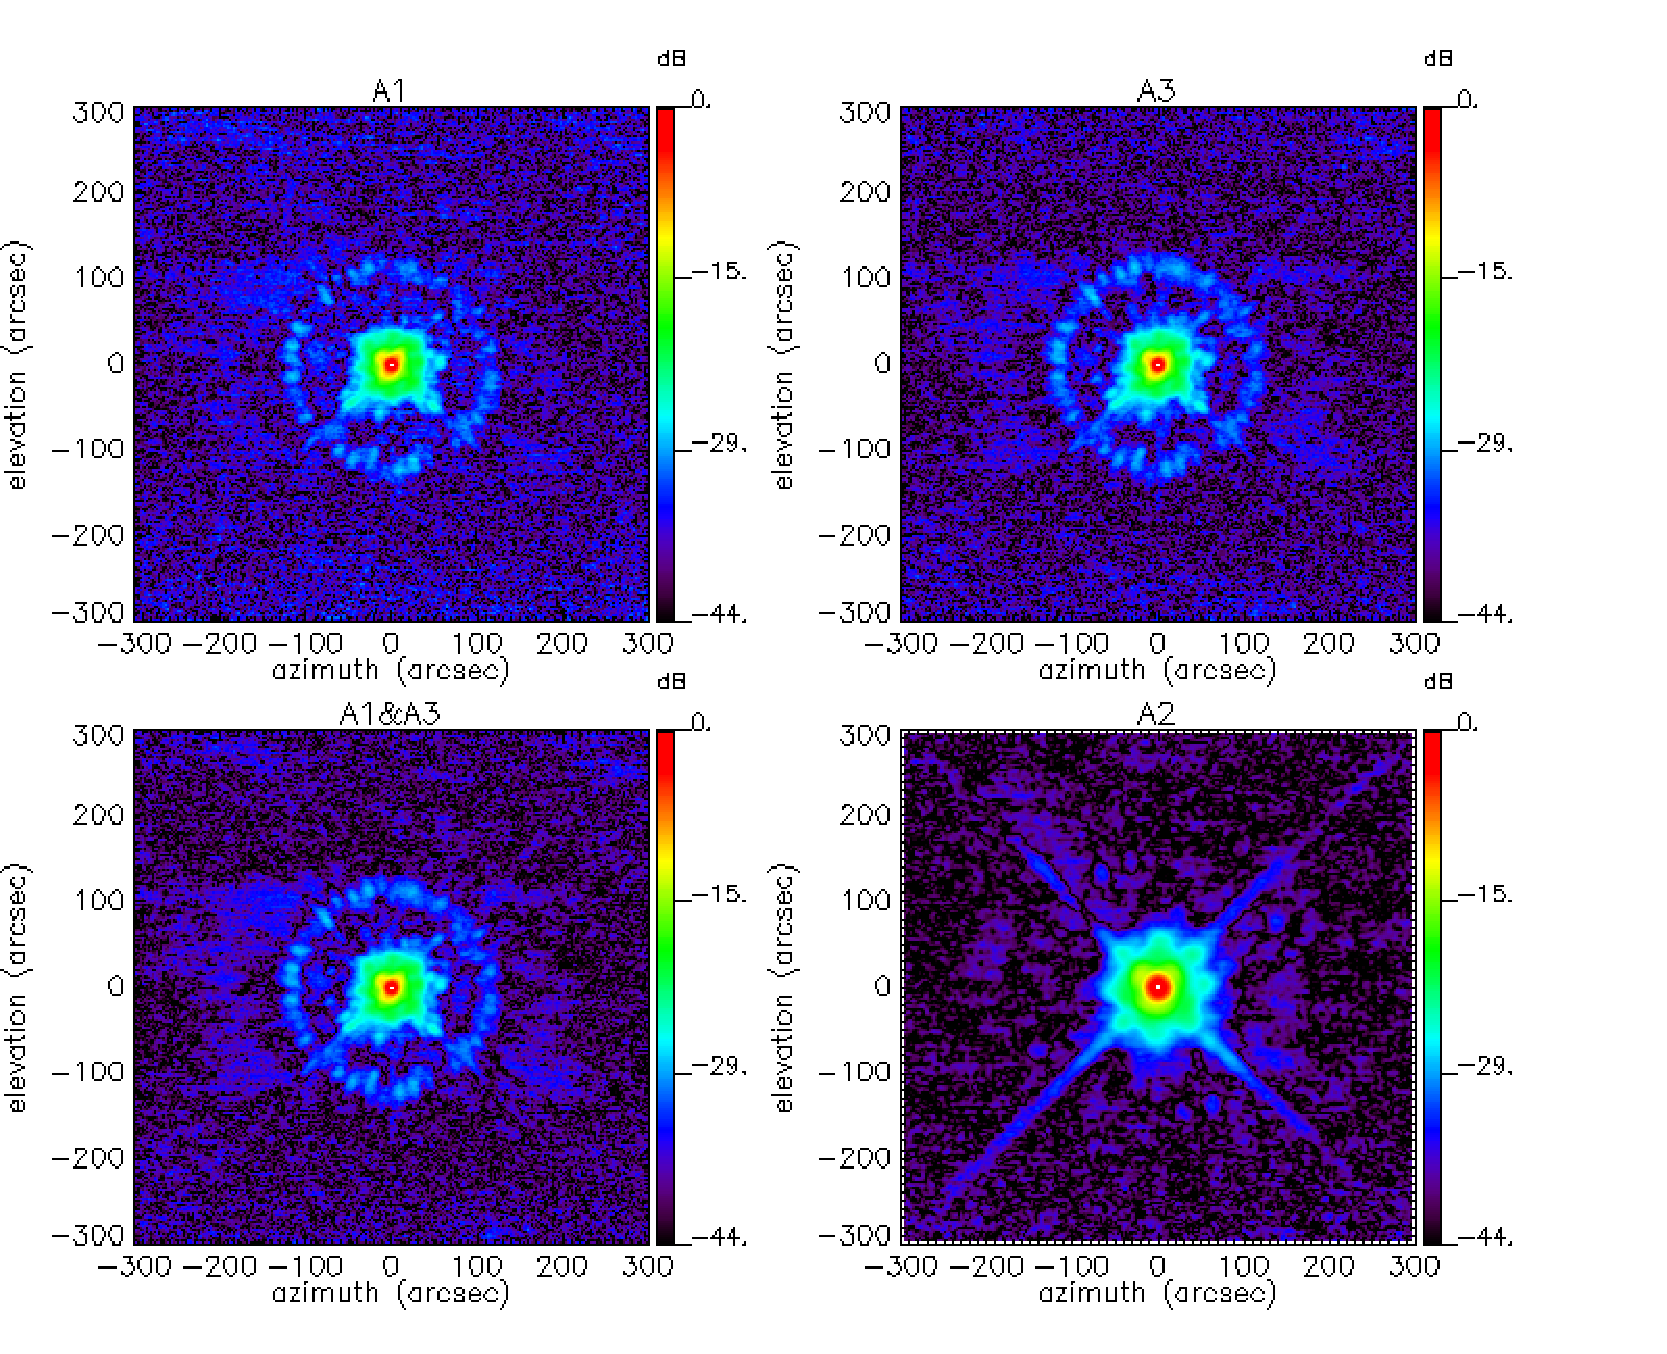
\includegraphics[clip, angle=0, scale=0.4]{Figures/Lobe_map_Combo_v2_dB.pdf}
 \caption[Beam pattern.]{From upper left to lower right, beam maps of array 1 (labeled 'A1'), array 3 ('A3'), the combination of the 1.15mm arrays ('A1$\&$3') and the 2mm array ('A2') are shown in decibel. These maps, which consist of normalized combination of four long OTF scans of bright point sources, are in celestial coordinates and cover a sky area which extend over 10 arcmin.}
\label{fig:beam}
\end{center}
\end{figure}


The deep NIKA2 beam maps reveal some noticeable features, which are
shown in Fig.~\ref{fig:features}.

{\bf Implement Samuel's comments copied below}
Commentaires faits a Alessandro pour le papier:
\begin{itemize}
\item[(1)] les four symmetrical spokes of the error beam sont normaux
  et attendu d'apres mes simus comme tu peux voir dans la petite image
  ci-dessous (c'est le beam obtenu dans Zemax pour la bande 1mm
  convolu\'e avec une fonction porte de la taille du pixel)
\item[(2)] par contre les pink ellipse show spikes in this map
  montrent un effet de diffraction ou de ghost image anormal et
  inattendu qui est du \'a un probleme optique dans le cryostat ou au
  niveau de M5 ou M6 ou la fenetre. On le sait car quand on regarde
  leur position en fonction de l'elevation on voit qu'ils tournent
  avec l'elevation dans les cartes Az-El
\item[(3)] quant aux spikes of unknown origin montr\'es sur A3 je pense
  que les deux en bas et a droite sont juste un des petits lobes de la
  simu avec un meilleur contraste que ceux du haut et de gauche, alors
  que pour le petit blob dans la diagonale a peu pres au niveau de
  la diffraction sur un bras du quadrupode je soupconne un effet
  d'amplification du a la petite boite qui se trouve sur le cot\'e du
  secondaire que tu peux voir sur la photo du slide 2 de la
  presentation qu'Andrea a envoyee aujourd'hui (mais je n'ai pas de
  preuve)
\end{itemize}



\begin{figure}
\begin{center}
  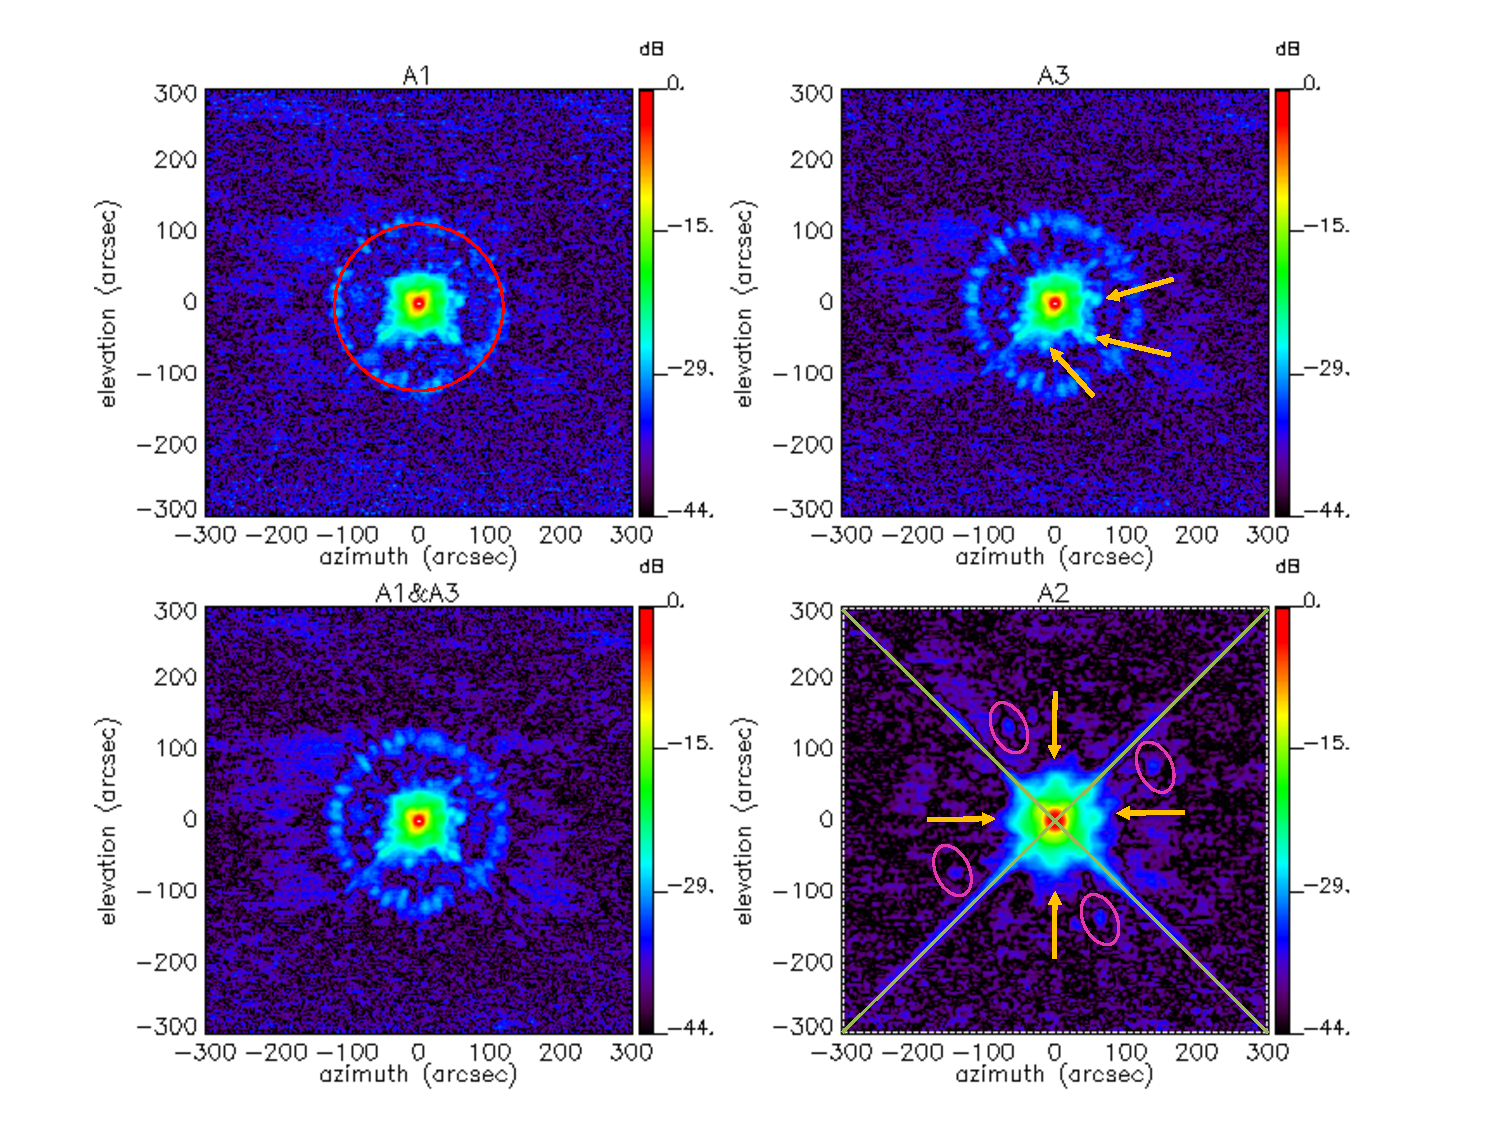
\includegraphics[clip, angle=0, scale=0.4]{Figures/Beams_features.pdf}
\caption[Noticeable features of NIKA2 beam pattern.]{ Red circle: diffraction ring seen in 1-mm maps (the spokes are presumably caused by radial and azimuthal panel buckling (cf. Fig.4 in Greve et al. 2010)); Perpendicular green lines: diffraction pattern caused by quadrupod secondary support structure (prominently seen in 2mm maps); Yellow arrows in the upper right pannel: pattern of 3 spikes seen in 1mm maps of unknown origin; Yellow arrows in the lower right pannel: four symmetrical spokes of the first errorbeam; Pink ellipses: 4 spikes seen in 2mm maps.}
\label{fig:features}
\end{center}
\end{figure}


To gain a first impression of the structure of the Iram 30-m beam as seen with NIKA2, we use radial cuts to evidence the relative level of the main beam, the first error beam and other features seen in the 2D beam pattern using radial cuts. NIKA2 full beam is shown in Fig.~\ref{fig:beam_db} by means of two orthogonal cuts through Uranus
from a high quality map obtained on 2017 January 25th in excellent conditions
(low opacity $\tau_{225}=0.08$ and elevation $46^{\circ}$).

\begin{figure}[h]
\begin{center}
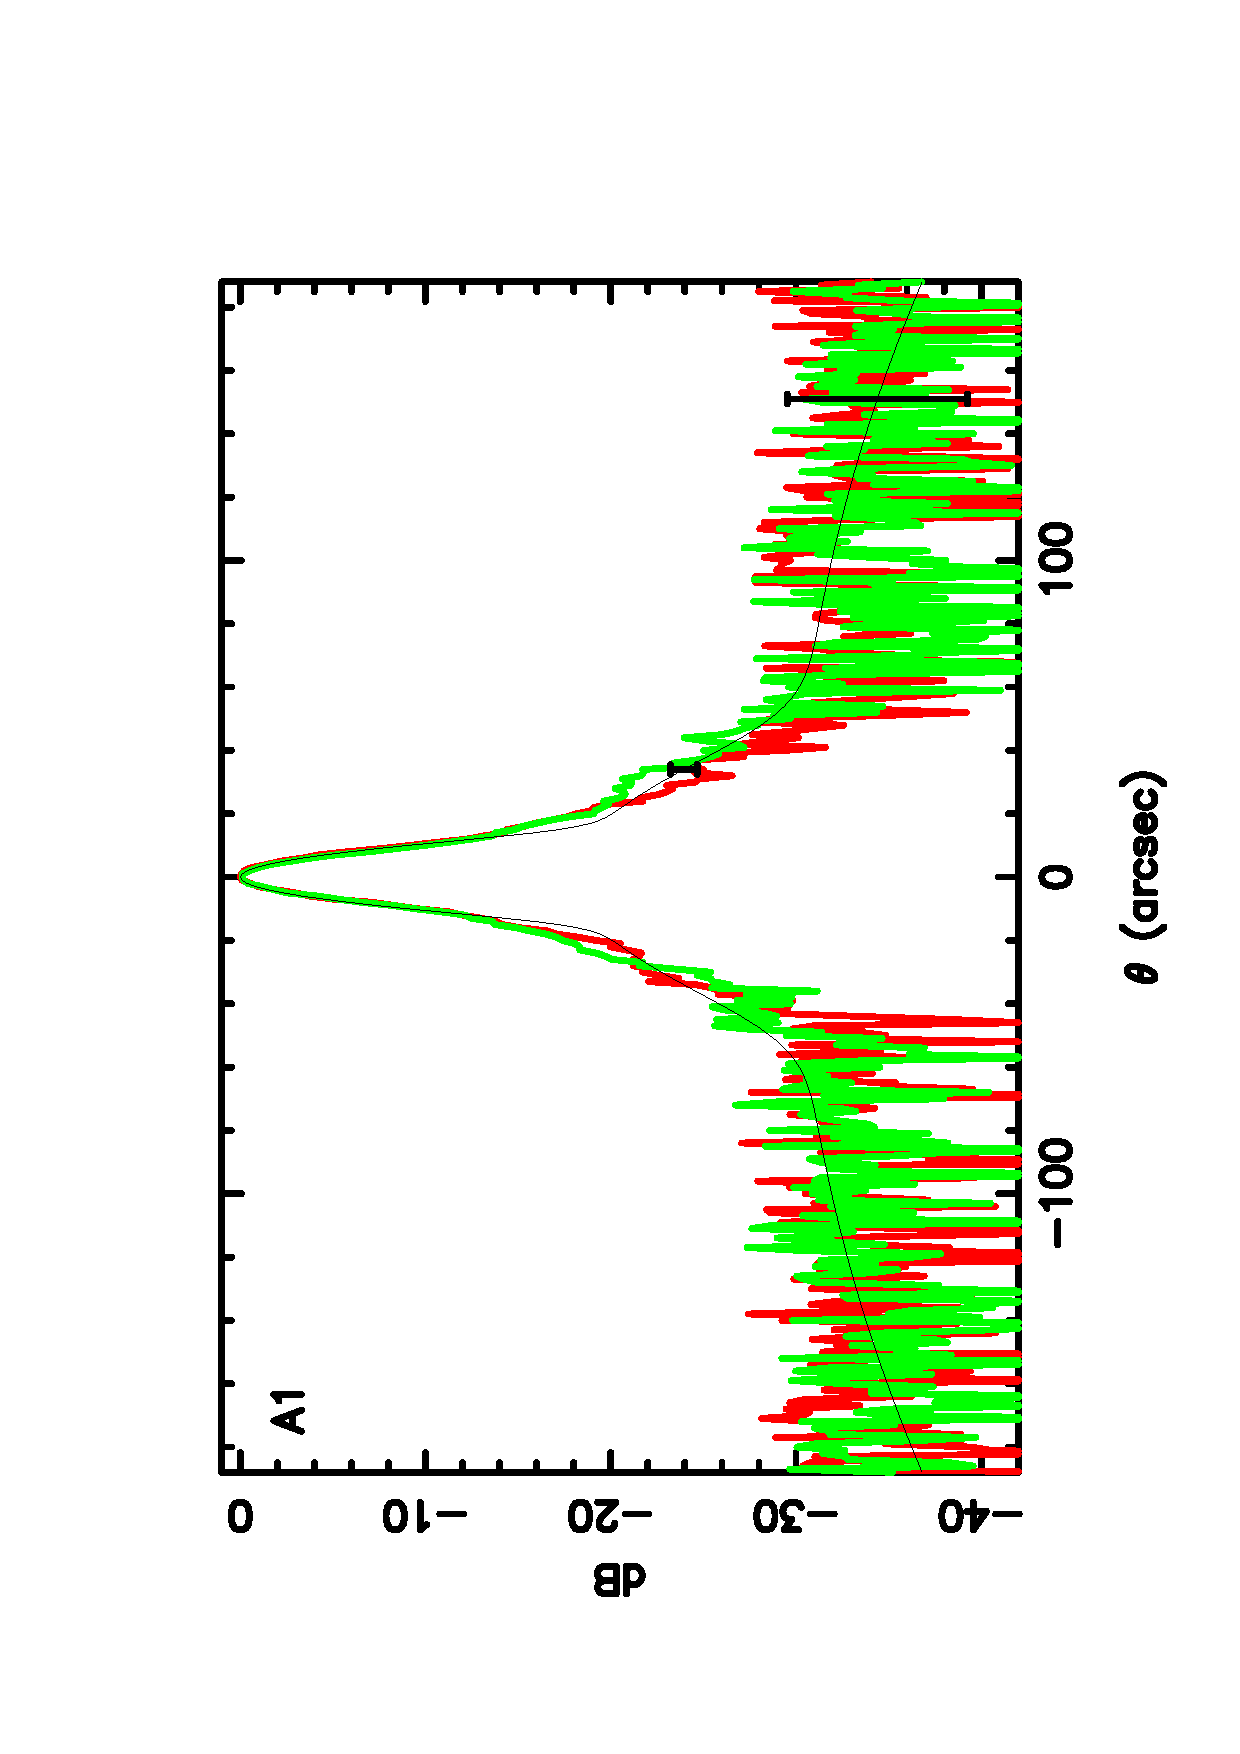
\includegraphics[clip, angle=-90, scale =0.3]{Figures/Array_A1_dB.pdf}
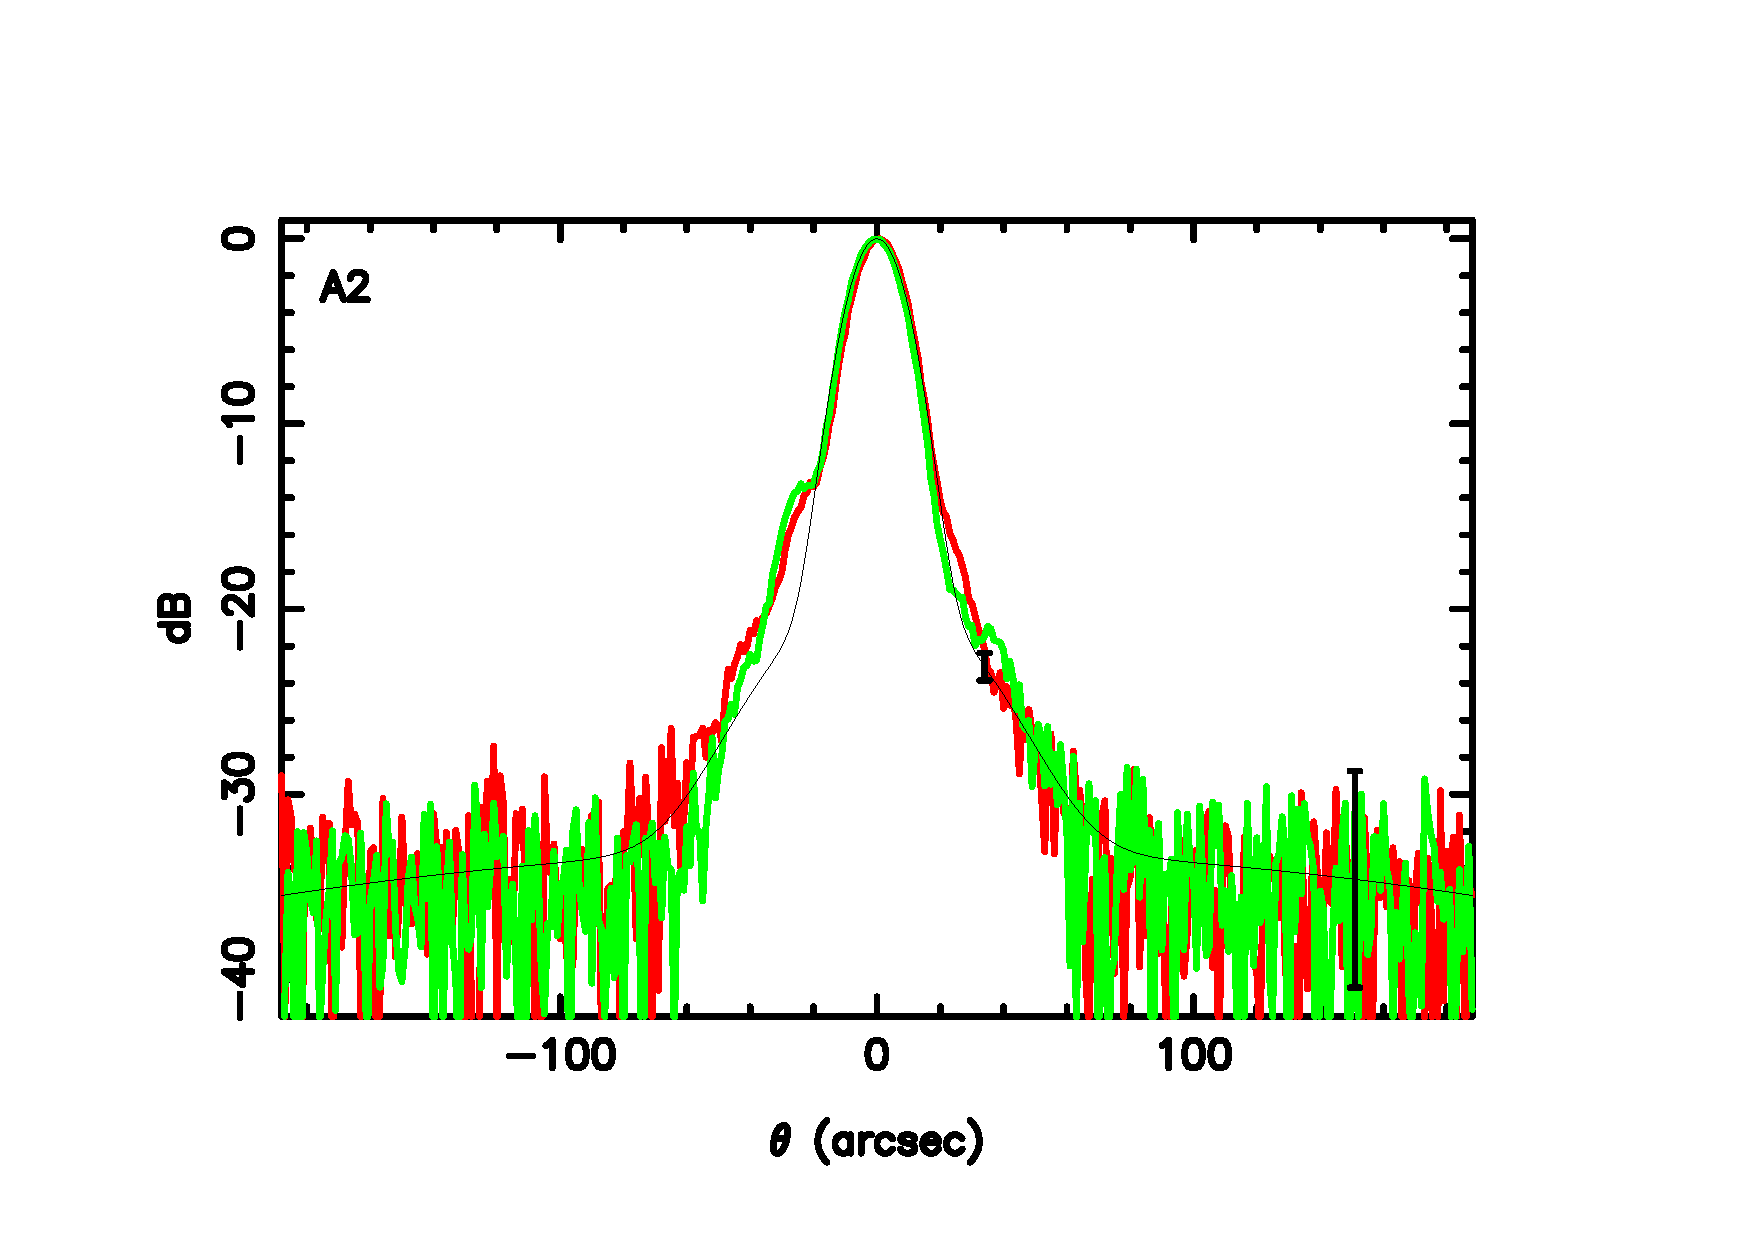
\includegraphics[clip, angle=-90, scale = 0.3]{Figures/Array_A2_dB.pdf}
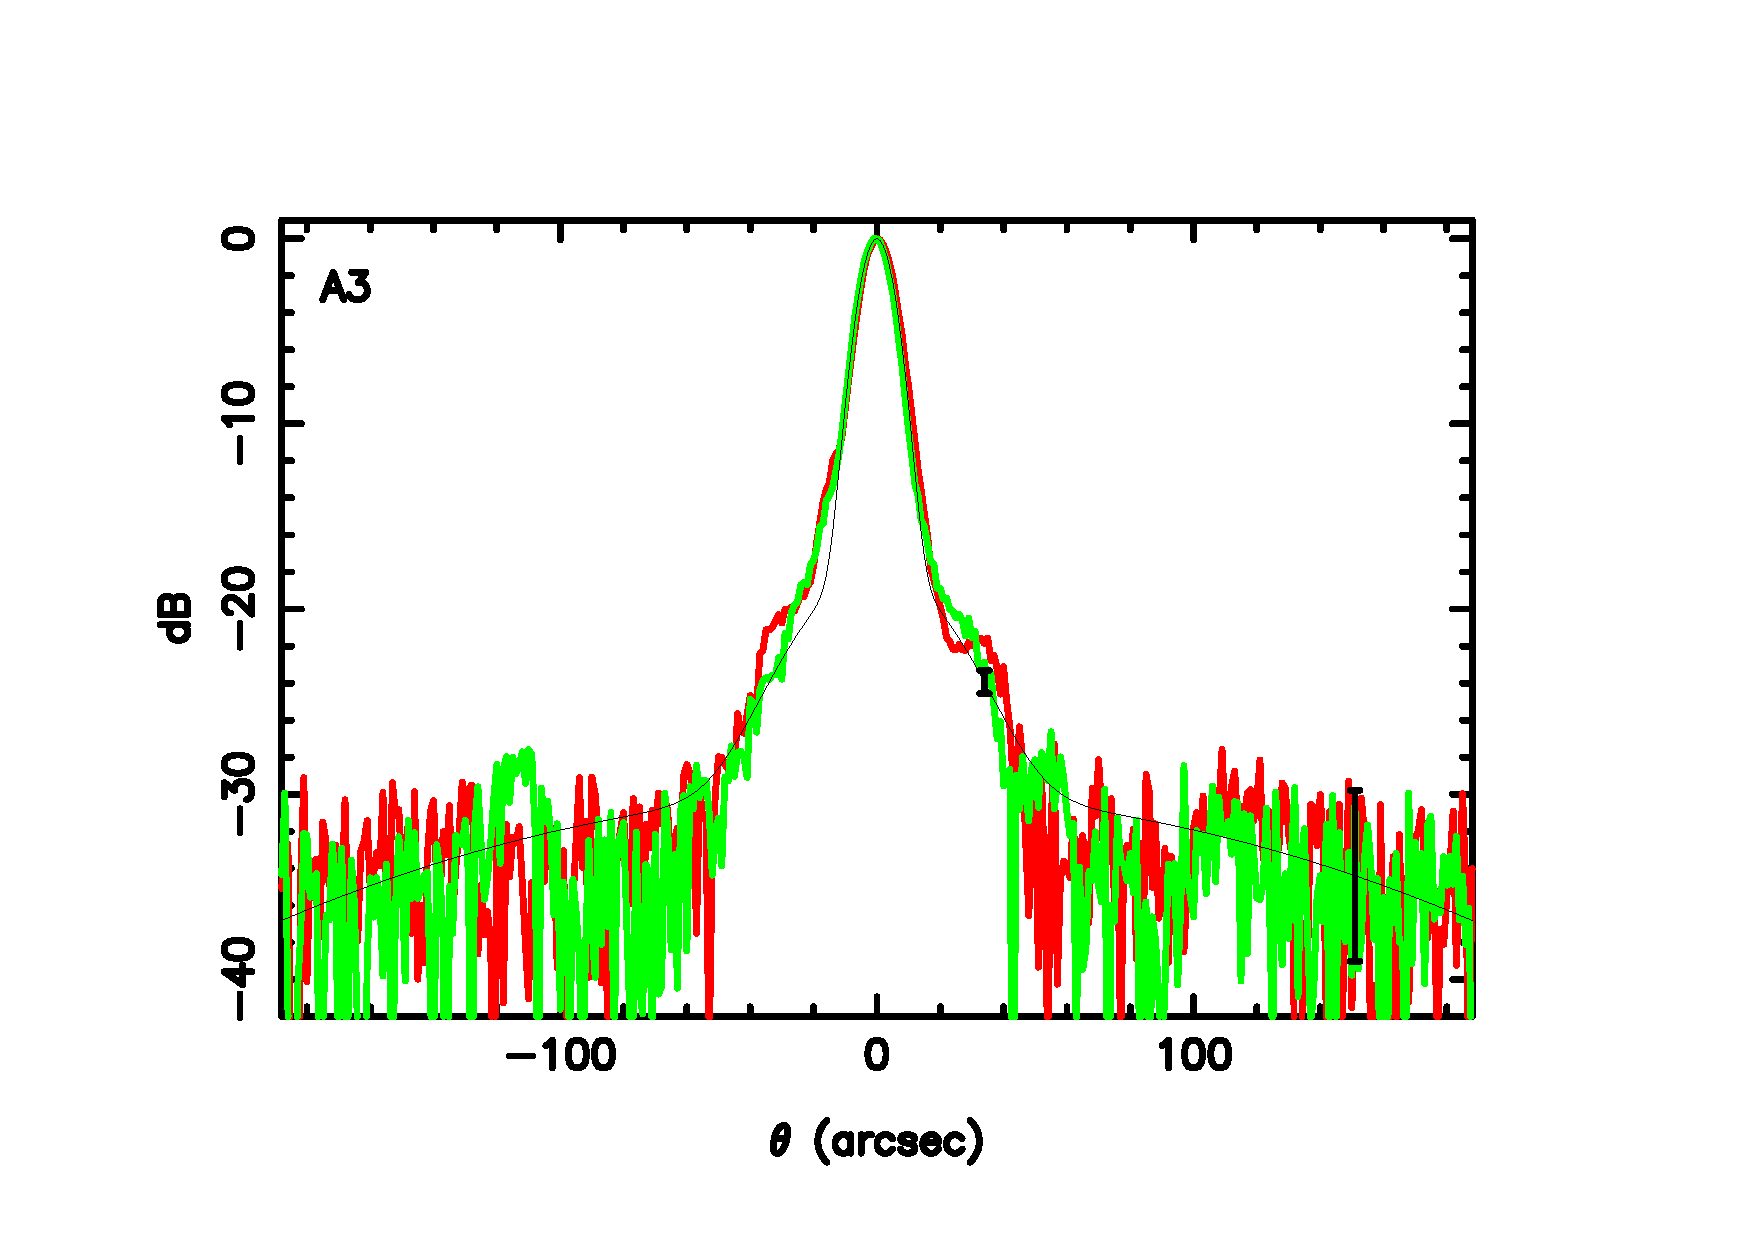
\includegraphics[clip, angle=-90, scale = 0.3]{Figures/Array_A3_dB.pdf}
\caption[Beam cuts]{Two orthogonal cuts through the beam are shown in red and green and a best fit model made
of three Gaussians is superimposed in black. These cuts were obtained from the high quality map of Uranus on 2017 January 25th.
The main beam starts to depart from the first Gaussian at -12dB. }
\label{fig:beam_db}
\end{center}
\end{figure}

A model made of three Gaussians centered on the source peak was best
fit {\it by hand} to these cuts.
%the parameters are reported in Table \ref{tab:3gauss} [PEUT-ETRE
%AVANTAGEUSEMENT REPLACED PAR VALEURS DE FLORIAN].
We observe that the main beam starts to depart from the first
Gaussian at the level of about -12dB for the three arrays.
We note that for the instrument EMIR on the radiotelescope,
this departure is about -20dB (Kramer, Penalver and Greve
2013). However, this
discrepancy between a feedhorn-based experiment and a bare pixels one
is expected since the main effect of the feedhorns is to lower the
side lobes of the Airy diffraction pattern.
The precise characterization of the full beam structure is discussed
in Sect.~\ref{se:fullbeam_prof}.  

%From parameters in Table \ref{tab:3gauss}, one can estimate that
%the source incident power is split about equally between the main beam
%and the error beam at 1mm, and these fractions are 70\% and 30\% at 2mm, respectively.
%This modelling uses the central
%region   $180'' \times 180''$ in size with a uniform noise rms from
%a larger area of 8' x 5' on the sky scanned with the arrays. It is expected
%that the error beam extend beyond these limits.


%\begin{table}
%\centering 
%\caption[]{Model parameters of the three Gaussian beam.}
%\begin{tabular}{|l|l|l|l|l|l|l|}
%\hline
%               & \multicolumn{3}{c|}{A1 and A3} & \multicolumn{3}{c|}{A2}  \\
%\hline
%fwhm      & $11.25''$ & $45''$  & $250''$ & $17.75''$ & $56''$  & $420''$ \\
%amplitude & 0.984     & 0.015   & 0.0005   &  0.9875   & 0.011   &  0.0005\\
%\hline
%\end{tabular}
%\label{tab:3gauss}
%\end{table}


\subsection{Beam profile}
\label{se:fullbeam_prof}

{\bf complete this sub-section}

The beam profile is the azimuthal average of the beam map around the
main beam center. Although the profile cannot represent the sub-dominant non-axisymetrical
extended features, which are seen in the beam pattern and discussed in
Sect.~\ref{se:beammaps} (telescope arms, spikes), it provides us with a useful
representation of the internal and central parts of the beam (about up to
$100''$). We determine a beam profile from a beam map in centering to
the fitted value of the main beam center and forming the
weighted average of the pixels equidistant to the center.

We model the beam profile as a three-Gaussian function defined as:
\begin{equation}
  B(\theta) = \sum_i A_i G_i(\theta) + B_0
\end{equation}


Figure \ref{fig:beam_profiles_3G} shows the beam profile from a beam
map acquired during {\emph N2R8} (scan ID: 20170125s223), as well as
the best-fit 3-Gaussian model. 

\begin{figure*}[h!]
\centering
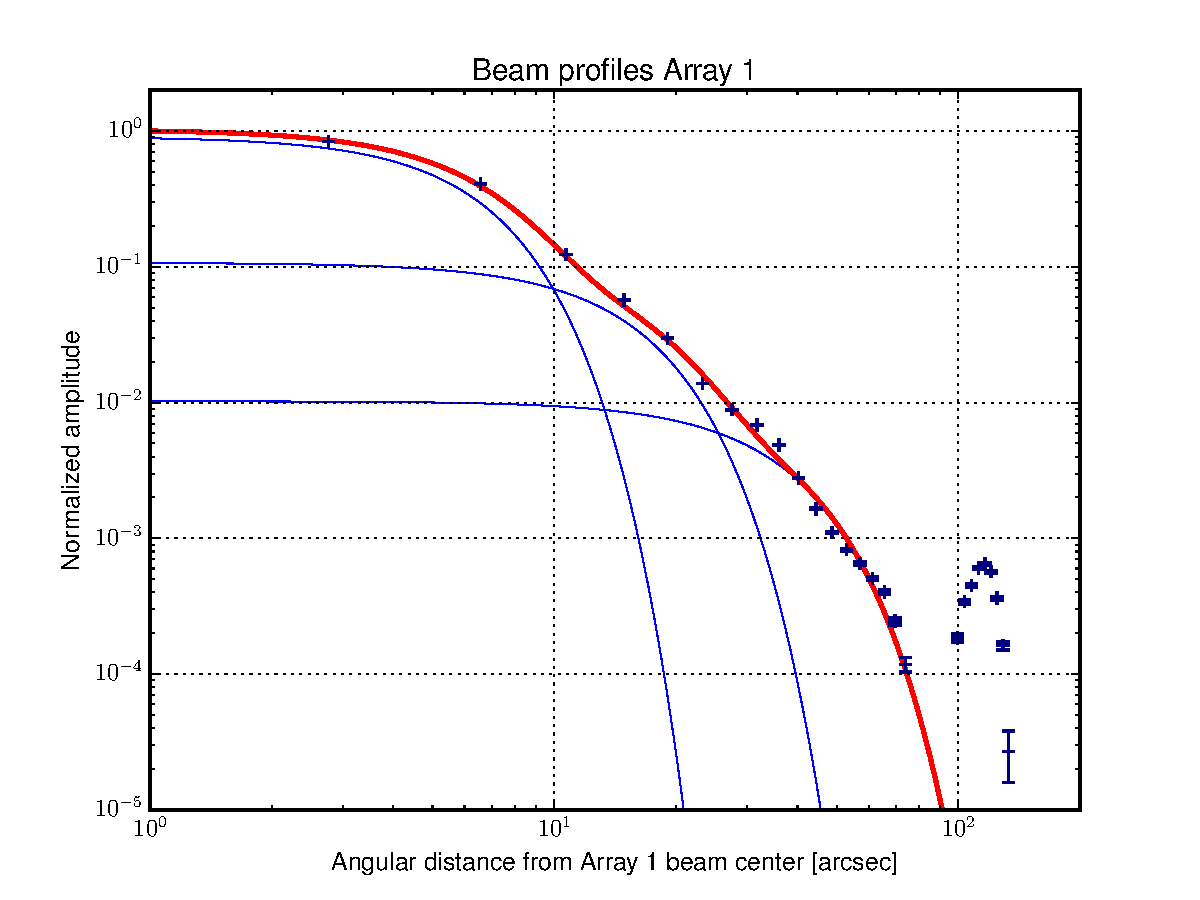
\includegraphics[height=6cm]{Figures/Beam_profiles_A1_FR.pdf}
\hspace{0.5cm}
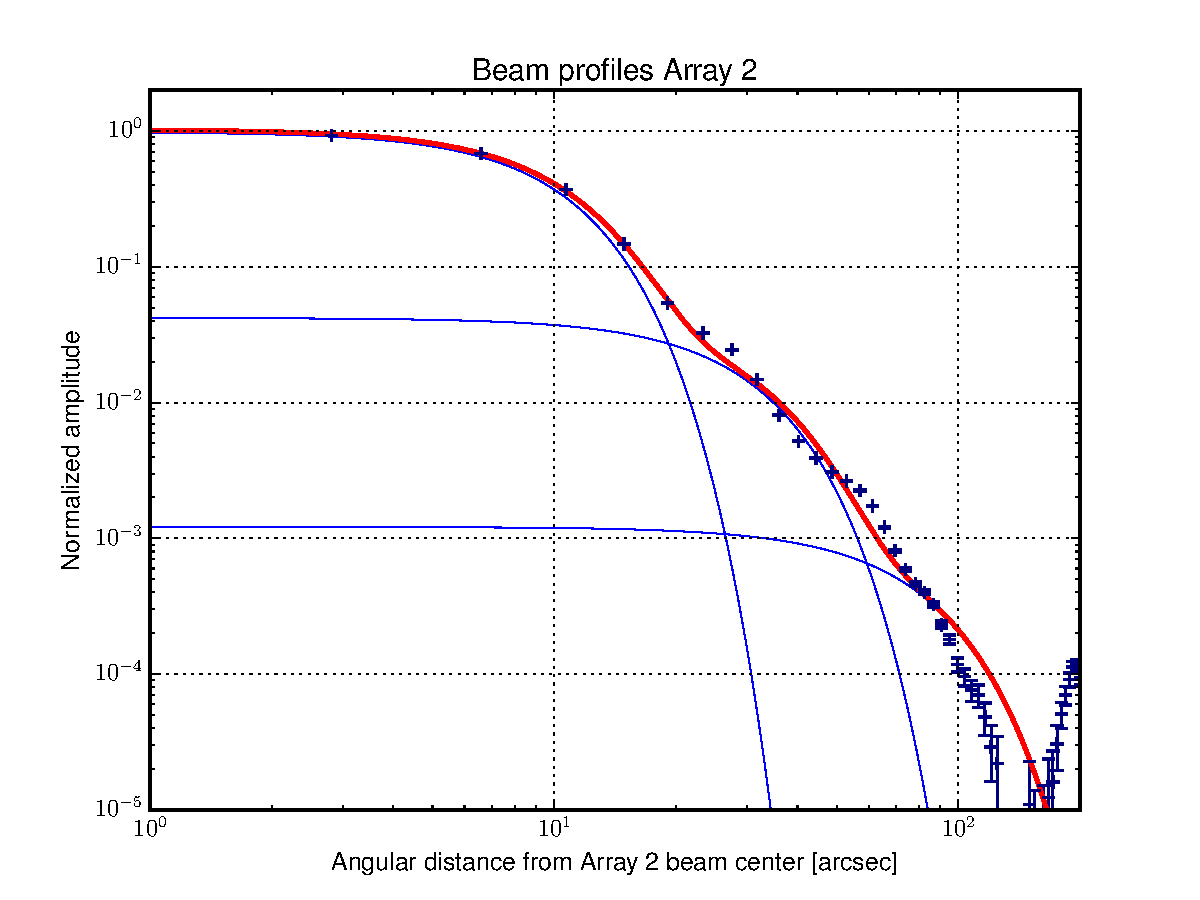
\includegraphics[height=6cm]{Figures/Beam_profiles_A2_FR.pdf}
\hspace{0.5cm}
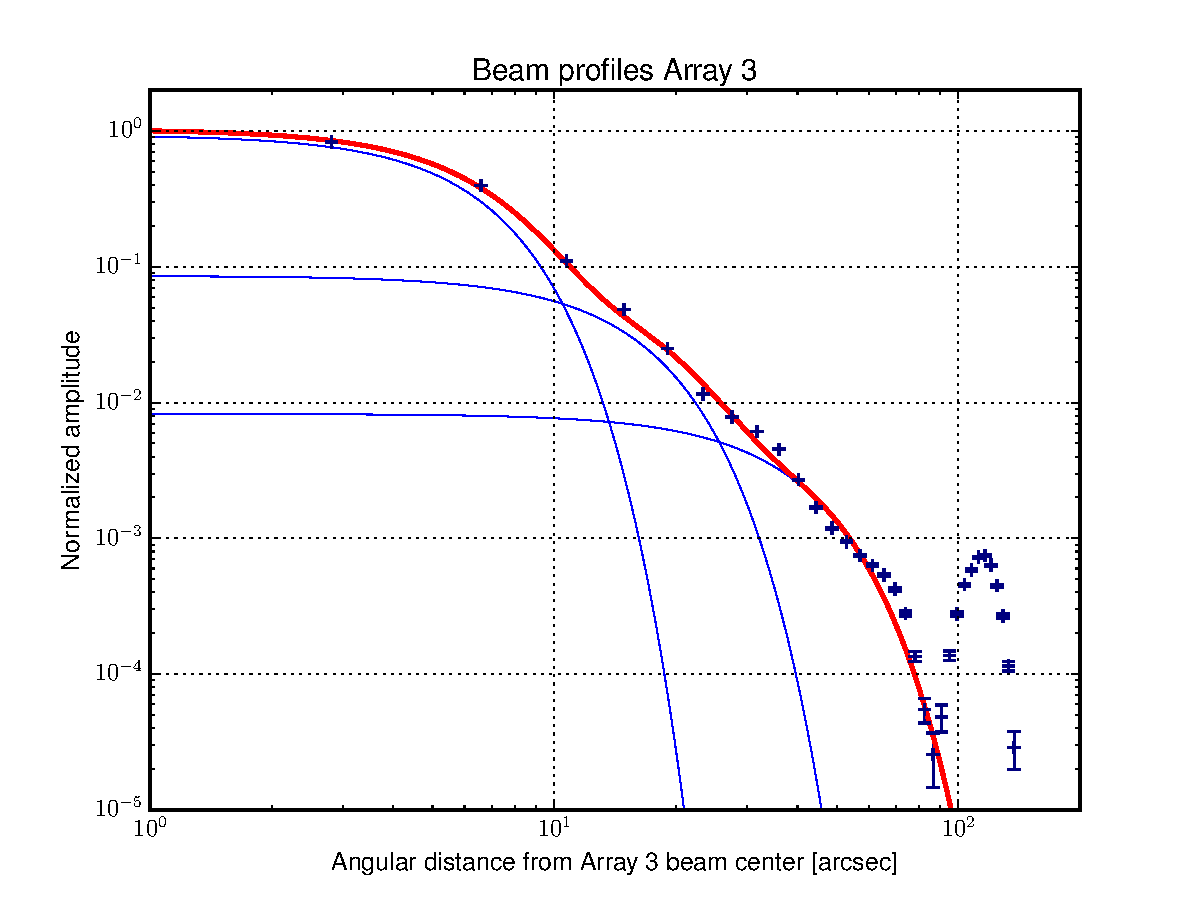
\includegraphics[height=6cm]{Figures/Beam_profiles_A3_FR.pdf}
\caption{Beam profiles for array 1, 2, and 3.}
\label{fig:beam_profiles_3G}
\end{figure*}

